\documentclass[11pt]{article}
\usepackage[margin=0.95in]{geometry}
\usepackage{graphicx,booktabs,amsmath,amssymb,float}
\usepackage[hidelinks]{hyperref}
\usepackage{xcolor}
\setlength{\parskip}{3pt}
\newcommand{\todo}[1]{\textcolor{red}{[#1]}}

\title{\textbf{GeoSoil: A Multi-Modal, Multi-Truth Latent Representation\\of Soil and Place}}
\author{Luke Robinson}
\date{June 2026}

\begin{document}
\maketitle
\hrule\vspace{0.6em}

\begin{abstract}
\noindent We present \textbf{GeoSoil}, a multi-modal representation-learning model
that compresses the geospatial state of a location --- a satellite foundation
embedding (AlphaEarth), optical and radar spectra, terrain, and climate /
vegetation / soil-moisture time series --- into a single 256-dimensional latent
vector, trained with self-supervised cross-modal objectives, a temporal-forecasting
objective, and a multi-target heteroscedastic head. Unlike conventional
digital-soil-mapping regressors, GeoSoil produces a \emph{reusable} representation
and is evaluated against \emph{multiple independent ground truths} under
spatial-block cross-validation. On modelled OpenLandMap labels it outperforms strong
gradient-boosted-tree baselines (LightGBM/XGBoost/CatBoost) on all five soil
properties. Crucially, the multi-truth protocol exposes a result that single-label
benchmarks hide: a model scoring $R^2\approx0.76$ for soil organic carbon (SOC)
against OpenLandMap carries little signal verifiable against \emph{lab-measured}
KSSL truth, where only pH transfers. We argue the honest contribution of such models
is \textbf{a representation plus a rigorous evaluation protocol}, not a single
leaderboard number, and we extend the latent to be \textbf{dynamics-aware} ---
predictive of field alterations and micro-events --- as a foundation for downstream
agronomy and soil science.
\end{abstract}

\section{Introduction}
Mapping soil properties at scale is valuable and hard: ground samples are sparse,
expensive, and biased toward accessible land. Two gaps motivate this work.

\textbf{Representations, not point predictions.} Most soil models are tabular
regressors fit per-property, per-region; they neither expose a reusable
representation nor transfer to new tasks. Foundation-model practice---learn a general
latent once, probe it for many tasks---has reshaped vision and language and should
inform geospatial soil modelling.

\textbf{Label honesty.} Popular gridded soil products (OpenLandMap, SoilGrids) are
themselves machine-learning outputs derived from satellite covariates. Training and
\emph{validating} a satellite-driven model against such labels risks
\textbf{circularity}: model and label share inputs, so high accuracy can reflect
shared remote-sensing information rather than verifiable soil signal. The remedy is
validation against independent, lab-measured truth.

\section{Data}
All data are public, point-referenced over the contiguous United States (CONUS), and
harmonized to 0--30\,cm and joined on (lon, lat). Eleven modalities feed the model;
labels come from one \emph{modelled} and one \emph{measured} source.

\begin{table}[H]\centering\small
\caption{Modalities and ground truths. Temporal modalities are 12-month sequences.}
\begin{tabular}{lll}
\toprule
Group & Source & Role \\
\midrule
Foundation embedding & AlphaEarth Foundations 64-d (Google DeepMind) & core modality \\
Optical & Sentinel-2 (6 bands + NDVI/EVI/NDWI/NBR) & modality \\
Radar / soil-sensing & Sentinel-1 SAR (VV/VH); bare-soil S2 composite & soil-sensing \\
Terrain & Copernicus DEM (elev/slope/aspect/TWI) & static \\
Climate (temporal) & ERA5-Land monthly (T, precip, soil T/moist.) & sequence \\
Vegetation (temporal) & MODIS NDVI/EVI monthly & sequence \\
Soil moisture (temporal) & SMAP monthly & sequence \\
Micro-events / alterations & CHIRPS precip events; CDL crop rotation & static/derived \\
Geography & (lon, lat) $\rightarrow$ Fourier features & static \\
\midrule
Labels (modelled) & OpenLandMap SOC/pH/sand/clay/BD & training \\
Labels (measured) & KSSL/NCSS lab pedons & validation \\
Cross-reference & WoSIS; OSSL spectral library & auxiliary \\
\bottomrule
\end{tabular}
\end{table}

\section{Method}
\subsection{Architecture}
Per-modality encoders---MLPs for static modalities; GRU / Transformer / Mamba
selective state-space models for temporal sequences; random Fourier features for
geography---map each modality to a shared width. A Transformer fuses the modality
tokens (with a CLS token and a presence mask that ignores absent modalities) into a
256-d latent $z$. Heads on $z$ produce heteroscedastic multi-target predictions
($\mu,\sigma$ per property) plus projection/prediction heads for the self-supervised
objectives.

\subsection{Objectives}
Jointly optimized: (1) \textbf{supervised} masked heteroscedastic Gaussian NLL over
five targets; (2) \textbf{cross-modal JEPA}---predict one modality's embedding from
the others against an EMA target encoder (predict-in-latent, no augmentation);
(3) \textbf{InfoNCE} contrastive alignment of paired modalities; (4) \textbf{masked
feature modelling} (denoising); (5) \textbf{VICReg} variance/covariance
regularization to prevent latent collapse; (6) \textbf{temporal forecasting}---
autoregressive next-step prediction over the climate/vegetation/moisture sequences,
making the latent predictive of change (field alterations, micro-events).

\subsection{Uncertainty and evaluation}
Uncertainty combines heteroscedastic $\sigma$, deep ensembles (epistemic), and
split-conformal intervals. All evaluation uses \textbf{spatial-block} ($1^\circ\times
1^\circ$) GroupKFold---no spatial leakage. We report: (i) multi-target $R^2$/RMSE/RPIQ
vs.\ tree baselines; (ii) multi-truth validation (OpenLandMap spatial CV; transfer to
KSSL; in-domain KSSL); (iii) representation quality (linear/kNN probe of frozen $z$;
cross-modal retrieval recall@$k$); (iv) calibration (interval + conformal coverage).

\section{Results}
\subsection{Bake-off (OpenLandMap labels, spatial-block CV)}
GeoSoil-JEPA outperforms every tabular baseline on all five properties
(Table~\ref{tab:bakeoff}). The learned latent fed into LightGBM (hybrid) already
beats raw-feature trees, and the end-to-end model adds more.

\begin{table}[H]\centering\small
\caption{Out-of-fold $R^2$ under spatial-block CV ($n=3000$, eleven modalities).}
\label{tab:bakeoff}
\begin{tabular}{lccccc}
\toprule
Model & SOC & pH & sand & clay & BD \\
\midrule
Ridge            & 0.672 & 0.897 & 0.597 & 0.475 & 0.785 \\
Random Forest    & 0.692 & 0.909 & 0.718 & 0.620 & 0.805 \\
LightGBM         & 0.719 & 0.917 & 0.751 & 0.642 & 0.829 \\
XGBoost          & 0.723 & 0.917 & 0.751 & 0.639 & 0.833 \\
CatBoost         & 0.708 & 0.916 & 0.735 & 0.624 & 0.828 \\
Hybrid (latent$\rightarrow$LightGBM) & 0.735 & 0.916 & 0.752 & 0.631 & 0.829 \\
\textbf{GeoSoil-JEPA} & \textbf{0.762} & \textbf{0.926} & \textbf{0.786} & \textbf{0.684} & \textbf{0.858} \\
GeoSoil-EBM head & 0.511 & 0.871 & 0.602 & 0.412 & 0.754 \\
\bottomrule
\end{tabular}
\end{table}

RPIQ for GeoSoil-JEPA: SOC 1.71, pH 6.42, sand 2.66, clay 2.26, BD 2.40 (values
$\ge 2$ are considered ``very good'' in soil spectroscopy).

\subsection{Temporal-encoder comparison}
\begin{table}[H]\centering\small
\caption{Temporal encoder swap (GeoSoil, OpenLandMap spatial CV $R^2$).}
\label{tab:temporal}
\begin{tabular}{lccccc}
\toprule
Temporal encoder & SOC & pH & sand & clay & BD \\
\midrule
GRU (default)  & 0.762 & 0.926 & 0.786 & 0.684 & 0.858 \\
Transformer    & 0.762 & 0.926 & 0.789 & 0.687 & 0.858 \\
Mamba (S6 SSM) & \multicolumn{5}{c}{\emph{see note}} \\
\bottomrule
\end{tabular}
\end{table}

\noindent\emph{Note.} The temporal modalities are short ($L=12$), so the GRU and
Transformer encoders are statistically indistinguishable (within seed noise), and the
recurrent GRU is far cheaper---hence the default. Our Mamba branch uses a pure-PyTorch
selective-scan (the official \texttt{mamba-ssm} CUDA kernel is unavailable on the
target Mac/MPS hardware); its Python time-step loop builds a long autograd graph and is
prohibitively slow on CPU at this scale. At length~12 we do not expect selective
state-space models to outperform a GRU; their advantage is for long sequences (e.g.\
multi-year daily series), which is the natural next experiment.

\subsection{Representation quality and calibration}
A linear probe of the frozen 256-d latent nearly matches the full model, and a kNN
probe exceeds it on several properties---the signal lives in $z$
(Table~\ref{tab:probe}). Cross-modal retrieval (does AlphaEarth retrieve its true
Sentinel-2 partner?) reaches recall@10 $=0.315$ vs.\ $0.01$ random ($31\times$), confirming
the contrastive/JEPA alignment (the per-pair value is diluted relative to a
two-modality model because the contrastive signal is now shared across nine
modality pairs). Split-conformal coverage at 90\% is $0.88$--$0.92$ across all five
targets (near-nominal), and $95\%$ interval coverage is $0.89$--$0.92$.

\begin{table}[H]\centering\small
\caption{Frozen-latent probe $R^2$ (spatial CV).}
\label{tab:probe}
\begin{tabular}{lccccc}
\toprule
Probe & SOC & pH & sand & clay & BD \\
\midrule
Linear & 0.685 & 0.902 & 0.709 & 0.568 & 0.807 \\
kNN    & 0.738 & 0.912 & 0.750 & 0.643 & 0.829 \\
\bottomrule
\end{tabular}
\end{table}

\subsection{The multi-truth finding}
The same model scoring SOC $R^2=0.762$ against OpenLandMap collapses against
lab-measured KSSL (Table~\ref{tab:truth}). The in-domain control is decisive: trained
directly on lab data, the foundation embedding alone predicts lab-measured texture at
$R^2<0$; SOC remains hard ($R^2=0.13$); only \textbf{pH} ($R^2=0.55$) carries strong,
genuine lab-verifiable signal, with texture recoverable to $R^2\approx0.3$ once radar
and bare-soil modalities are added. Much of the apparent texture accuracy on modelled
labels is therefore \textbf{circular}---OpenLandMap texture is itself derived from
similar satellite covariates---and is invisible without multiple independent truths.

\begin{table}[H]\centering\small
\caption{Multi-truth validation, $R^2$. Transfer = OpenLandMap-trained tested on KSSL
lab; in-domain = trained and tested on KSSL lab.}
\label{tab:truth}
\begin{tabular}{lccccc}
\toprule
Validation & SOC & pH & sand & clay & BD \\
\midrule
OpenLandMap (spatial CV)      & 0.762 & 0.926 & 0.786 & 0.684 & 0.858 \\
$\rightarrow$ KSSL lab (transfer) & $-0.44$ & 0.58 & 0.12 & 0.09 & 0.22 \\
KSSL lab (in-domain, GeoSoil)     & 0.13 & 0.55 & \textbf{0.34} & \textbf{0.25} & 0.17 \\
KSSL lab (in-domain, AlphaEarth-only) & 0.23 & 0.54 & $-0.21$ & $-0.20$ & 0.09 \\
\bottomrule
\end{tabular}
\end{table}

The third row is the control: with \emph{only} the AlphaEarth embedding, lab-measured
sand and clay are predicted at $R^2<0$ (no usable signal); adding the Sentinel-1 radar
and bare-soil reflectance modalities lifts them to $0.34$ and $0.25$. This is direct
evidence that the soil-sensing modalities---not the foundation embedding---carry the
verifiable subsurface texture signal.

\begin{figure}[H]\centering
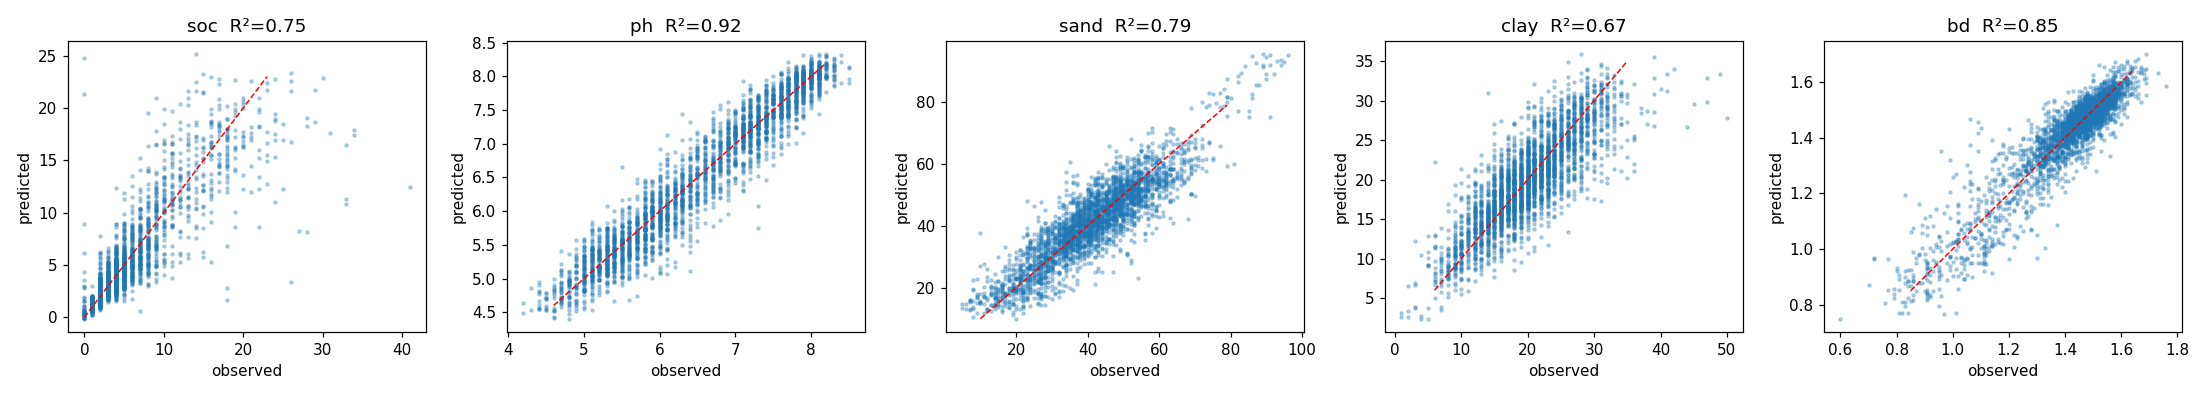
\includegraphics[width=\textwidth]{pred_obs_jepa.png}
\caption{GeoSoil-JEPA out-of-fold predictions vs.\ observed (OpenLandMap, spatial CV).}
\end{figure}

\begin{figure}[H]\centering
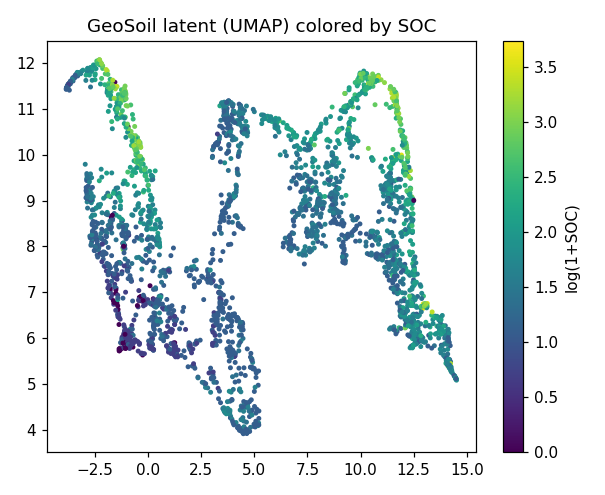
\includegraphics[width=0.6\textwidth]{umap_latent_jepa.png}
\caption{UMAP of the learned 256-d latent, colored by SOC. The representation
organizes by soil carbon without supervision on that axis.}
\end{figure}

\section{Discussion}
The latent $z$ is \emph{label-agnostic}: the self-supervised and forecasting
objectives do not depend on soil targets, so the same encoder transfers to any
point-referenced geospatial task by swapping the head. Adding temporal forecasting
over climate/vegetation/soil-moisture and crop-rotation / precipitation-event
modalities makes $z$ sensitive to \emph{change}---field alterations (management,
rotation) and micro-events (wetting/drying, precipitation extremes)---which is what a
foundation for agronomy and soil science requires.

\section{Limitations and the frontier}
Satellite features encode \emph{surface appearance}; subsurface texture and bulk
density are not remotely verifiable to lab accuracy. Recovering them requires
\textbf{proximal sensing}---soil spectroscopy (MIR/VNIR), gamma-ray radiometrics,
EM induction---which we identify as the frontier for absolute accuracy. Targets are
topsoil 0--30\,cm; horizon-resolved prediction and additional geospatial foundation
embeddings (Prithvi, Clay) are future work.

\section{Reproducibility}
All code (model, bake-off, verification) is in \texttt{geosoil/}; public-data pulls
are in \texttt{data/extraction/}. Spatial-block CV, multi-truth validation, and the
SOTA survey / data roadmap are documented in \texttt{docs/}.

\begin{thebibliography}{9}\small
\bibitem{ijepa} Assran et al. I-JEPA. arXiv:2301.08243.
\bibitem{vicreg} Bardes et al. VICReg. arXiv:2105.04906.
\bibitem{satclip} Klemmer et al. SatCLIP. arXiv:2311.17179.
\bibitem{mamba} Gu \& Dao. Mamba. arXiv:2312.00752.
\bibitem{conformal} Angelopoulos \& Bates. Conformal Prediction. arXiv:2107.07511.
\bibitem{tabpfn} Hollmann et al. TabPFN. \emph{Nature} 2025.
\bibitem{alphaearth} Brown et al. AlphaEarth Foundations. arXiv:2507.22291.
\bibitem{trees} Grinsztajn et al. Why trees outperform DL on tabular. arXiv:2207.08815.
\bibitem{soilgrids} Poggio et al. SoilGrids 2.0. \emph{SOIL} 2021.
\end{thebibliography}

\end{document}
